
\documentclass[paper=a4, fontsize=11pt]{scrartcl} % A4 paper and 11pt font size

\usepackage[T1]{fontenc} % Use 8-bit encoding that has 256 glyphs
\usepackage{fourier} % Use the Adobe Utopia font for the document - comment 
\usepackage[english]{babel} % English language/hyphenation
\usepackage{amsmath,amsfonts,amsthm} % Math packages
\usepackage{graphicx}
\usepackage{float}
\usepackage{subfig}
\usepackage{caption}
\usepackage[section]{placeins}
\usepackage{sectsty} % Allows customizing section commands
\allsectionsfont{\centering \normalfont\scshape} 
\numberwithin{equation}{section} 
\numberwithin{figure}{section} 
\numberwithin{table}{section} 

\setlength\parindent{2pt} 
%-------------------------------------------------------------------------------
%	TITLE SECTION
%-------------------------------------------------------------------------------

\newcommand{\horrule}[1]{\rule{\linewidth}{#1}} 

\title{	
\normalfont \normalsize 
\textsc{PH 481 Lab} \\ [25pt] 
\horrule{2pt} \\[0.5cm] % Thin top horizontal rule
\huge Optics Lab 7\\ % The assignment title
\horrule{2pt} \\[0.5cm] % Thick bottom horizontal rule
}

\author{Harsukh Singh} % Your name

\date{\normalsize \today} % Today's date or a custom date

\begin{document}

\maketitle % Print the title
\section{Overview of Experiment}
This lab was focused on polarization of light. It was set up in the usual U type geometry for most optics experiments and the light source was aligned to the rail as usual. There was one polarizer set up as a polarizer of the incoming light and the other was set up as a analyzer, the set up of this is shown below.
\begin{figure}[H]
\centering
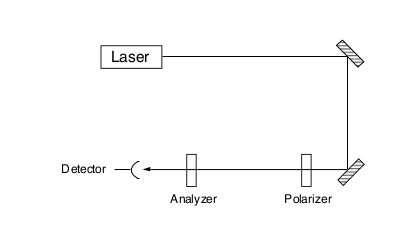
\includegraphics[scale =0.4]{stage}
\caption{Set Up}
\end{figure}
\section{Law of Malus}
The Law of Malus is used to describe the intensity of light coming from a linear polarizer as a function of angle $\theta$ between the polarizer transmission axis and the plane of polarization can be desribed by,
\begin{equation}
I(\theta) = I_0cos^2(\theta)
\end{equation}
With the aligned optical rail we set up the outcoming light from the analyzer to start at the first minimum (finding this experimentally). The first minimum was observed at $\theta = 120 ^{\circ}$. From the first minimum we vary the angle in steps of 10 degrees until the next minimum is observed. The experimental vs theoretical plots of this shown below,
\begin{figure}[H]
\centering
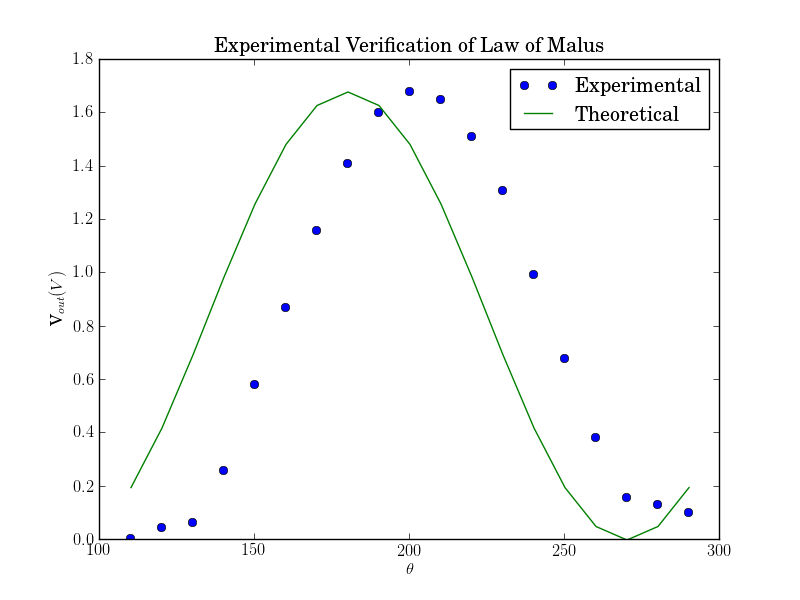
\includegraphics[scale =0.4]{malus}
\caption{Experimental vs Theoretical for Malus's Law}
\end{figure}
from what is observed above one can see that there is a phase shift between the experimental and theoretical plots. This primarily comes from measurement error from the experiment. This could be reduced by taking smaller step sizes in the polarizer and less interference from the incoherent light source (the room light) and better alignment from the optical equipment. 
\section{Linearly Polarized Light and Interference from Microscope Slide}
In this section we found the brewster angle of the glass slide and switched the incoming light to s-polarization from the lab instructions. However the second part does not have enough data because the interference pattern could not be observed.
\section{Absorption of Materials}
In this part of the lab we used a spectrometer to the measure the transmission of light through colored slides and also measured the transmission and reflection of a thin film.

\subsection{Colored Slide}
We calibrated the spectrometer so that the it was set to zero the natural light of the room. We passed light through the various slides and observed the plots of the transmission shown below.
\begin{figure}[H]
\centering
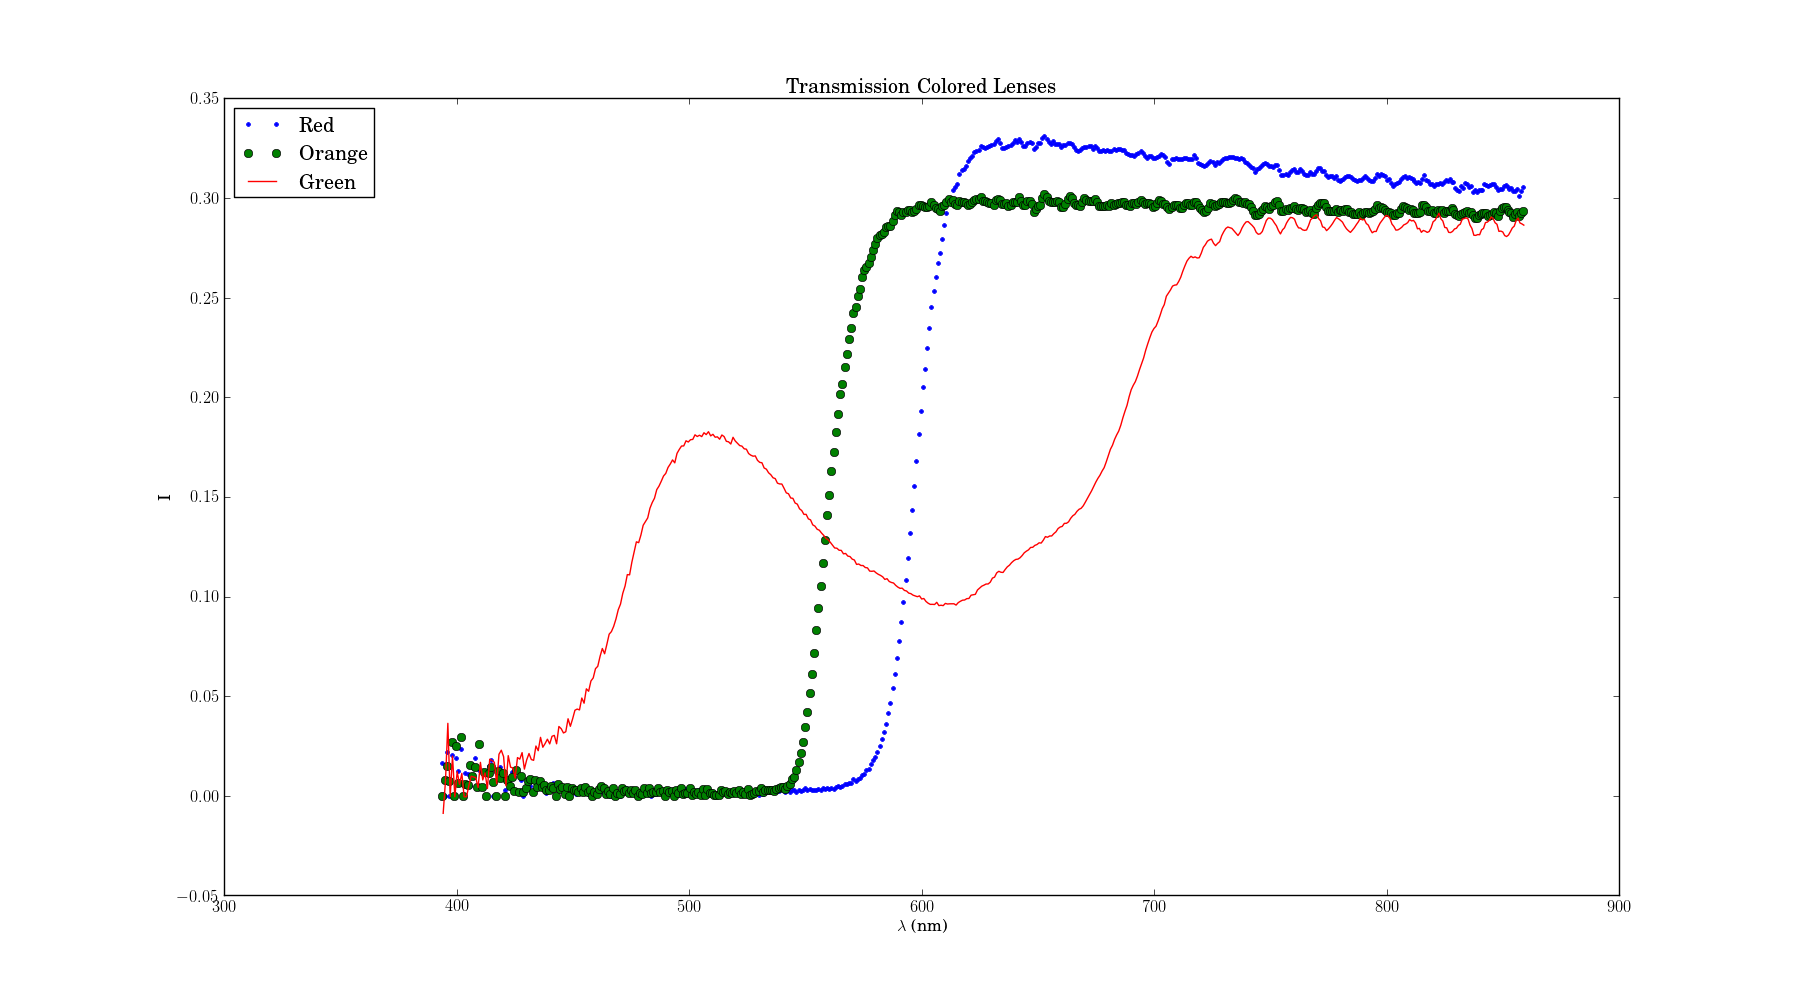
\includegraphics[scale =0.3]{lenses}
\caption{Transmission of light through colored slides}
\end{figure}
From figure 4.1 we can see that the tranmission function corresponds to the wavelength of the particular color. So the transmission only allows the wavelength of the color or higher through or stated another way, the light that gets transmitted through the material will show only those wavelengths of light that are not absorbed. 

\subsection{Thin Films}
In this part of the experiment we wanted to find the thickness of a thin film on the properties of the reflection and transmission. We can plot the the absorption of the thin film using Beer-Lambert Equation given below,

\begin{equation}
\alpha(\lambda) = \frac{-ln(\frac{T}{1-R})}{d}
\end{equation}
from the lab we know that the thin film has a thickness of 243 nm, so $d = 243 nm$.
so the plot of the absorption coefficient is shown below.
\begin{figure}[H]
\centering
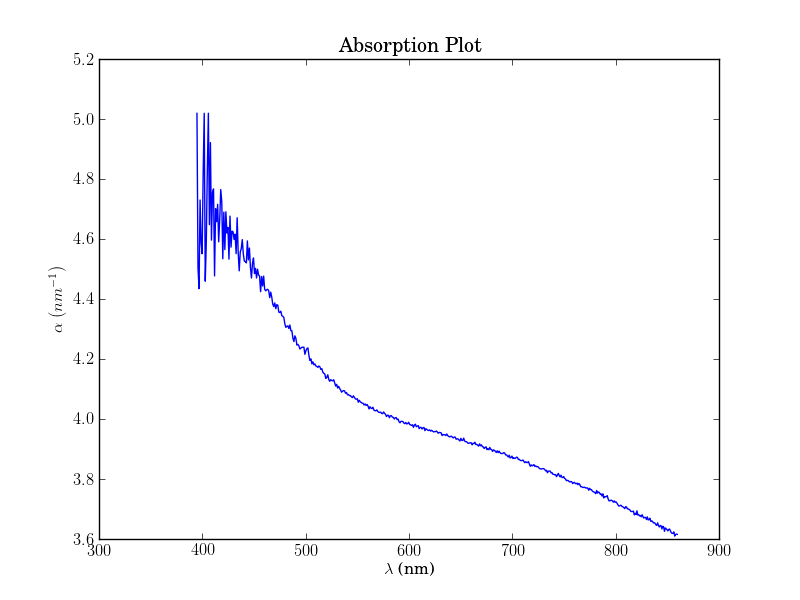
\includegraphics[scale =0.3]{abs}
\caption{Absorption coefficient in thin film}
\end{figure}
The light is absorbed mostly at lower wavelengths and has a high peak at the somewhere around 420 nm. 
\section{Conclusion}
Although I did not get to the second the interference in the microscope slide. The interference pattern can be explained by 9.37 in Hecht on Dielectric films and the derivation follows from the book, thus it wasn't included.
\end{document}

%\begin{figure}[htb]
%\centering
%\parbox{5cm}{
%\includegraphics[width=5cm]{figure_1}
%\caption{ Reflection Coefficients}}
%\qquad
%\begin{minipage}{5cm}
%\includegraphics[width=5cm]{figure_2}
%\caption{Transmission Coefficients}
%\end{minipage}
%\end{figure}
%
%\begin{figure}[htb]
%\centering
%\parbox{5cm}{
%\includegraphics[width=5cm]{Epar}
%\caption{Electric Field Parallel to Incident Plane}
%\label{fig:2figsA}}
%\qquad
%\begin{minipage}{5cm}
%\includegraphics[width=5cm]{Eperp}
%\caption{Electric Field Perpendicular to Indicent Plane}
%\label{fig:2figsB}
%\end{minipage}
%%\end{figure}
%
%\section{Experiment 1.1:  Transmittance through Glass}
%\begin{figure}[!ht]
%	\caption{Experimental Set-Up}
%		\begin{center}
%			\includegraphics[scale=0.5]{transmittance}
%		\end{center}
%\end{figure}

%\begin{figure}[!ht]
%	\caption{Experimental Comparison to Theoretical Transmission 
%Coefficients}
%		\begin{center}
%			\includegraphics[scale=0.5]{figure_3}
%		\end{center}
%\end{figure}
%
%\section{Experiment 1.2:  Reflectance from Frosted Glass}
%\begin{figure}[!ht]
%		\begin{center}
%			\includegraphics[scale=0.5]{reflectance}
%		\end{center}
%\caption{Reflectance from Frosted Glass}
%\end{figure}

%\section{Experiment 1.3: Refraction through glass slab}
%\begin{figure}[!ht]
%		\begin{center}
%			\includegraphics[scale=0.5]{GlassLab}
%		\end{center}
%\caption{Measuring the index of refraction through Glass Slab}
%\end{figure}g
% \begin{equation}
%sin(\theta_i -\theta_t) = \frac{l}{\frac{t}{cos(\theta_t)}}
% \end{equation}
% and,
% \begin{equation}
%n_{slab}  = 
%\frac{n_1sin(\theta_1)}{sin(\theta_1-sin^{-1}(\frac{t}{\frac{l}{sin(\theta_i 
%-\theta_t)}}))}
% \end{equation}
% Solving this $n_{slab} = 1.42$  and since most glass has a refractive index 
% of ~1.5 this was pretty close.
% \begin{equation}
%   \begin{tabular}{|l |r| }
%     \hline
%      d(m) & 0.0065561             \\ \hline
%     d^{'} (m) & 0.0064660        \\ \hline
%     d^{''}(m) & 0.006345             \\  \hline
%     d^{'''}(m)& 0.0061452               \\  \hline
%   \end{tabular}
% \end{equation}
% \begin{figure}[htb]
% 	\caption{Fabry-Perot fringes (I vs delta)}
% 		\begin{center}
% 			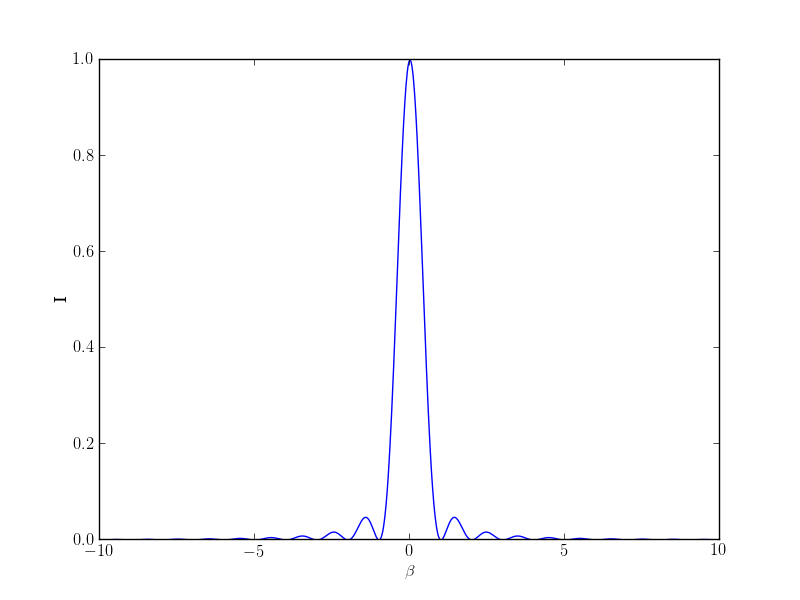
\includegraphics[scale=0.5]{fringes}
% 		\end{center}
% \end{figure}
% \begin{table}[H]
%   \centering 
%    \caption{data}
%   \begin{tabular}{|l |r| }
%     \hline
%      3 slits & $\frac{2}{3}$ \\ \hline
%      4 slits & $\frac{2}{4}$ \\ \hline
%      10 slits & $\frac{2}{3}$ \\  \hline
%   \end{tabular}
% \end{table}
% \begin{figure}[H]
% \centering
% 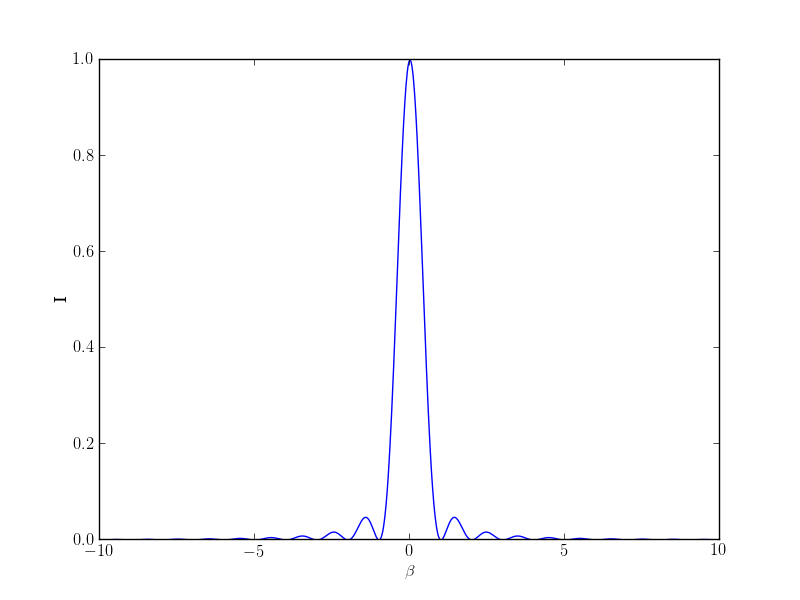
\includegraphics[scale =0.4]{fringes}
% \caption{Irradiance}
% \end{figure}
